%------------------------------------------------------------------------------------
%	CHAPTER 3
%------------------------------------------------------------------------------------
\chapterimage{headerCap.jpeg}
\chapter{Quebrar a Cabeça}

\begin{remark}
	Você não é Assembly mas eu quebro muito a cabeça para te entender. (Davyd Maker) 
\end{remark}

\section{Aprendizado e desafios}\index{Quebrar a Cabeça}
Quando era mais jovem e iniciei no mundo da programação propus uma vez um desafia para mim, deveria fazer determinada coisa com a linguagem que escolhesse se conseguisse estava em bons caminhos, caso contrário, bem tentar novamente. Ou seja, era um desafio que não tinha muita saída, realizava ou realizava. Fosse ele fazer um programa para mostrar uma determinada figura na tela ou mesmo aprender a utilizar vetores. 

Ou seja fazia algo que muitas pessoas consideravam idiota (achou que ia falar impossível) e talvez realmente fosse, mas idiota no sentido de não ser algo prático para se utilizar, mas era meu modo de criar um "Hello World" mais inteligente. Nessa seção teremos meus quatro desafios básicos, e se posso quero lhe sugerir que tente resolvê-los antes de ler a solução. Veja qual é o desafio, entenda o requisito e resolva-o depois pode ver a solução. Vou lhe dar uma dica preciosa antes mesmo de começarmos, escreva no papel o que pretende fazer e organize suas ideias, senão conseguir organizá-las então isso não serve como programa.

Para todos os programas utilizaremos a biblioteca apenas com o conjunto do segmento data (de modo que possamos escrever os nomes e não os códigos) e o arquivo makefile para compilar e linkeditar, então se acostume a copiá-los para cada um dos programas descritos e que seja seu ponto de partida.

\section{Programa 3.1 - Quadrado}\index{Quebrar a Cabeça}
Com base em um determinado valor mostrar um quadrado de asteriscos. Como disse, as pessoas consideravam desafios idiotas pois nunca teremos um usuário pedindo: "Me dê um quadrado de asteriscos". Esse desafio é excelente para aprendermos a controlar estruturas de repetição determinada aninhas (vulgo comando "for" dentro de outro "for"). 
\begin{figure}[H]
	\centering
	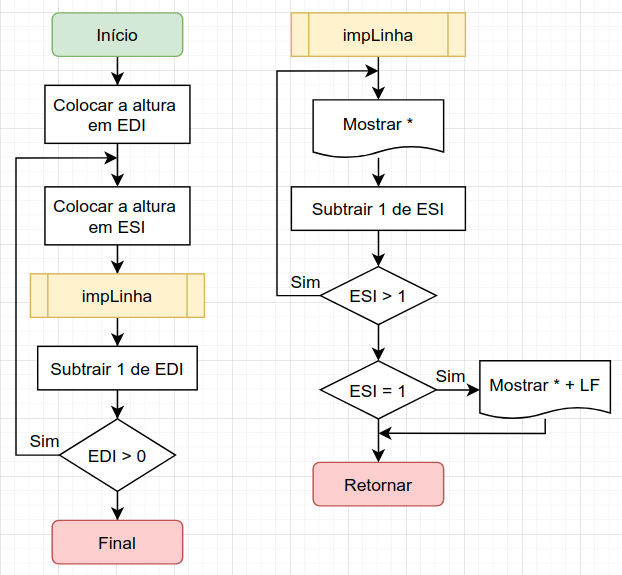
\includegraphics[width=0.6\textwidth]{Pictures/cap03/programa31}
	\caption{Fluxograma do Programa \textbf{Quadrado}}
\end{figure}

Criar um arquivo chamado "quadrado.asm" e começamos com a seguinte codificação:
\begin{lstlisting}[]
%include 'bibliotecaE.inc'

SECTION .data
  estrela DB '*', LF, NULL
  altura EQU 4

SECTION .text

global _start
\end{lstlisting}

Começamos então com a definição da nossa cadeia de caracteres para a saída e do valor da altura. Montamos o corpo principal:
\begin{lstlisting}[]
_start:
  mov edi, altura

inicio:
  mov esi, altura
  call impLinha
  sub edi, 0x1
  cmp edi, 0x0
  je saida
  jmp inicio	
\end{lstlisting}

Colocamos o valor da altura em \textbf{EDI} (que controla a quantidade de linhas), para o marcador \textbf{inicio}, colocamos o valor da altura em \textbf{ESI} (que controla a quantidade de colunas), saltamos para um marcador de modo a mostrar 1 linha, reduzimos a quantidade de \textbf{EDI} e comparamos seu valor com 0, se for igual vamos para o marcador \textbf{saida} caso contrário retornamos para o marcador \textbf{início}.

\begin{lstlisting}[]
impLinha:
  call impEstrela
  sub esi, 0x1
  cmp esi, 0x1
  jg impLinha
  je impEstrelaFinal
  ret
\end{lstlisting}

No marcador \textbf{impLinha} mostramos um * na saída do terminal, reduzimos o valor de \textbf{ESI} e verificamos se este for maior que 1 retornamos para o marcador \textbf{impLinha}, se for igual mostramos "* + LF" (para saltar de linha) e retornamos para o ponto que nos chamou.

\begin{lstlisting}[]
saida:
  mov eax, SYS_EXIT
  mov ebx, EXIT_SUCESS
  int SYS_CALL	
\end{lstlisting}

Neste ponto apenas fazemos as movimentações para terminar o programa. Mas calma que ainda existem mais dois marcadores importantes no conjunto.

\begin{lstlisting}[]
impEstrela:
  mov eax, SYS_WRITE
  mov ebx, STDOUT
  mov ecx, estrela
  mov edx, 0x1
  int SYS_CALL
  ret	
\end{lstlisting}

Observe que a cadeia de caracteres estrelas é formada por 3 elementos, dois deles é que nos interessam, se enviamos o tamanho em 1 apenas estamos tratando de mostrar '*' na saída do terminal e o cursor ficará na mesma linha, sem "cair" para a próxima.

\begin{lstlisting}[]
impEstrelaFinal:
  mov eax, SYS_WRITE
  mov ebx, STDOUT
  mov ecx, estrela
  mov edx, 0x2
  int SYS_CALL
  ret	
\end{lstlisting}

Já neste pedimos para mostrar o tamanho de dois que contém o '*' com Line Feed (ou quebra de linha se prefere) e assim ao mostrar o '*' desce para a próxima linha. Podemos agora imprimir quadrados de vários tamanhos, bastando apenas alterar a variável \textbf{altura}.

\section{Programa 3.2 - Pirâmide}\index{Quebrar a Cabeça}
Criar uma pirâmide de Asteriscos com base no valor da altura, por exemplo, se essa for 3 a pirâmide deve ser mostrada da seguinte forma:
\begin{lstlisting}[]
  *
 ***
*****
\end{lstlisting}

Para um valor 4, sairá assim:
\begin{lstlisting}[]
   *
  ***
 *****
*******
\end{lstlisting}

O que mais gosto desse desafio é que apresenta um elemento que não estamos vendo, os espaços iniciais, temos aqui duas perguntas que devemos resolver:
\begin{enumerate}[nolistsep]
	\item Quantidade de espaços em brancos em cada linha?
	\item Quantidade de * adicionados a cada 2ª linha?
\end{enumerate}

Pensemos assim, se a altura passada for 5, na primeira linha quantos espaços em branco iniciais temos? Isso mesmo 4, mas essa é a resposta errada, na verdade temos a altura menos 1 (já que estamos na 1ª linha), na segunda linha a resposta não muda, é a altura menos 2 (agora estamos na 2ª linha). Agora vamos focar na segunda pergunta, temos 1 na 1ª linha, e são adicionados mais 2 asteriscos a cada linha.

\begin{figure}[H]
	\centering
	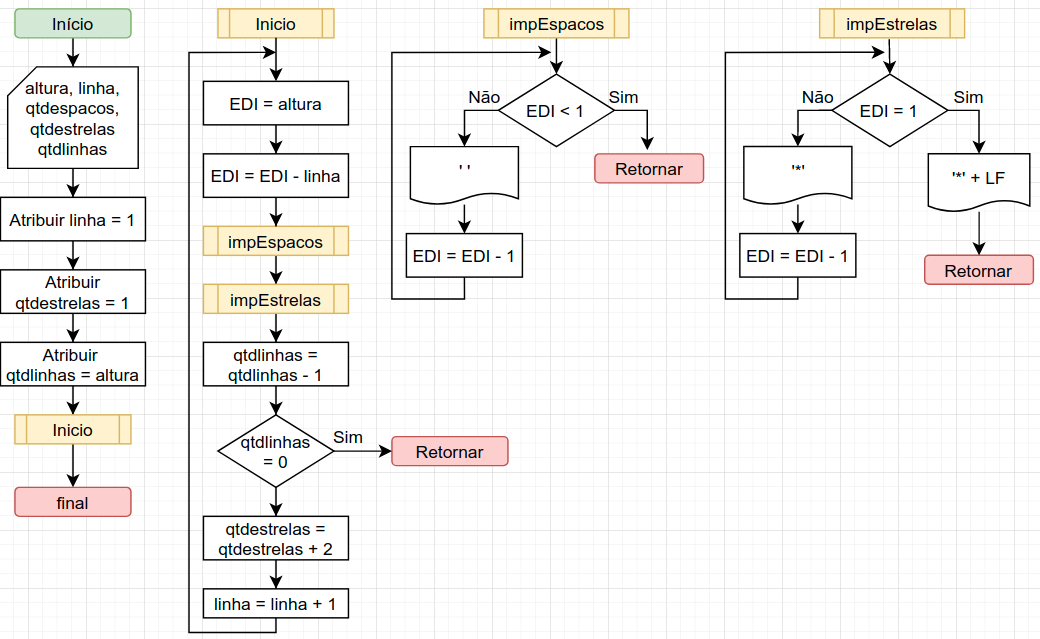
\includegraphics[width=0.75\textwidth]{Pictures/cap03/programa32}
	\caption{Fluxograma do Programa \textbf{Pirâmide}}
\end{figure}

Criar um arquivo chamado "piramide.asm" e começamos com a seguinte codificação:
\begin{lstlisting}[]
%include 'bibliotecaE.inc'

SECTION .data
  estrela  DB  '*', LF, NULL
  espaco   DB  ' ', LF, NULL

SECTION .bss
  altura      resb 0xA ; Altura (fixa)
  linha       resb 0xA ; linha atual
  qtdespacos  resb 0xA ; Qtd de espacos
  qtdestrelas resb 0xA ; Qtd de estrelas
  qtdlinhas   resb 0xA ; Qtd linhas ja impressa

SECTION .text

global _start
\end{lstlisting}

Essa é a parte fácil: Codificar. Trata apenas de uma simples tradução para o nosso fluxograma que já escrevemos. Gostaria muito que as pessoas observassem que NUNCA podemos iniciar a codificação se primeiro não temos as respostas para nosso problema, seria uma simples perda de tempo (ou se prefere tentativa e erro).E falando sério, é por isso que existem tantas piadas a respeito de programas errados ou de programadores fazendo besteiras pois eles preferem encurtar o caminho.

Seguimos agora para o início do marcador \textbf{\_start} no qual atribuímos os valores as nossas variáveis:
\begin{lstlisting}[]
_start:
  mov byte[altura], 0x8
  mov byte[linha], 0x1
  mov byte[qtdestrelas], 0x1
  mov byte[qtdlinhas], 0x8
\end{lstlisting}

No marcador \textbf{inicio} é que temos o coração do nosso programa:
\begin{lstlisting}[]
inicio:
  mov edi, dword[altura]
  sub edi, dword[linha]
  call impEspacos
  mov edi, dword[qtdestrelas]
  call impEstrelas
  sub byte[qtdlinhas], 0x1
  cmp byte[qtdlinhas], 0x0
  je saida
  add byte[qtdestrelas], 0x2
  add byte[linha], 0x1
  jmp inicio	
\end{lstlisting}

Movemos para \textbf{EDI} o valor da altura e subtraímos da linha atual (resposta da 1ª pergunta) e mostramos os espaços. Movemos para \textbf{EDI} o valor da quantidade de estrelas e mostramos os asteriscos. Reduzimos um na quantidade de linhas e verificamos se chegou a 0 para terminamos, caso contrário, adicionamos mais dois asteriscos na quantidade e mais um a linha atual e saltamos para o início do marcador.

\begin{lstlisting}[]
impEspacos:
  cmp edi, 0x1
  jl finalImpEspaco
  call impEspaco
  sub edi, 0x1
  jmp impEspacos
  
finalImpEspaco:
  ret  	
\end{lstlisting}

Para mostrar os espaços basta verificarmos o registrador \textbf{EDI} que contém a quantidade que deve ser mostrado, para isso logo no início já o comparamos com um e se for menor chamamos o marcador \textbf{finalImpEspaco} que retorna para quem nos chamou (isso é feito pois reparemos que na última linha não existe nenhum espaço). Saltamos para o marcador que vai mostrar um único espaço, reduzimos um na quantidade de \textbf{EDI} e retornamos para o início desse marcador.

\begin{lstlisting}[]
impEstrelas:
  cmp edi, 0x1
  je impEstrelaFinal
  call impEstrela
  sub edi, 0x1
  jmp impEstrelas	
\end{lstlisting}

Mais um marcador de controle, agora para a impressão dos asteriscos, basicamente a mesma coisa do anterior porém com a diferença que ao término devemos imprimir o asterisco que conterá o salto de linha. De resto temos uma repetição padrão do anterior.

\begin{lstlisting}[]
saida:
  mov eax, SYS_EXIT
  mov ebx, EXIT_SUCESS
  int SYS_CALL	
\end{lstlisting}

E finalmente a saída do programa e encerramento das chamadas. Espera um pouco não faltou mais 3 marcadores? Sim, dois deles vimos no programa anterior:
\begin{lstlisting}[]
impEstrela:
  mov edx, 1
  mov ecx, estrela
  mov eax, SYS_WRITE
  mov ebx, STDOUT
  int SYS_CALL
  ret

impEstrelaFinal:
  mov edx, 2
  mov ecx, estrela
  mov eax, SYS_WRITE
  mov ebx, STDOUT
  int SYS_CALL
  ret
\end{lstlisting}

Que mostra o asterisco na mesma linha e o asterisco com o salto de linha, e agora basta apenas repetir o primeiro marcador, mas ao invés de usarmos o asterisco vamos usar o espaço.
\begin{lstlisting}[]
impEspaco:
  mov edx, 1
  mov ecx, espaco
  mov eax, SYS_WRITE
  mov ebx, STDOUT
  int SYS_CALL
  ret	
\end{lstlisting}

E estamos prontos para mostrarmos uma pirâmide de qualquer tamanho possível, recomendo que tente estender este programa para mostrar um "Losango" (basta inverter a pirâmide). 

% Final do Capítulo
\clearpage